\chapter{Chiffrement RSA}

\section{Écrire un programme d'exponentiation rapide}

L'exponention rapide est une méthode permettant de calculer rapidement des grandes puissances de nombre. En effet, pour calculer de manière simple $n^p$ avec $p$ très grand, c'est-à-dire en multipliant $n$ par lui-même $p$ fois, est très peu efficace.

Un algorithme plus efficace 

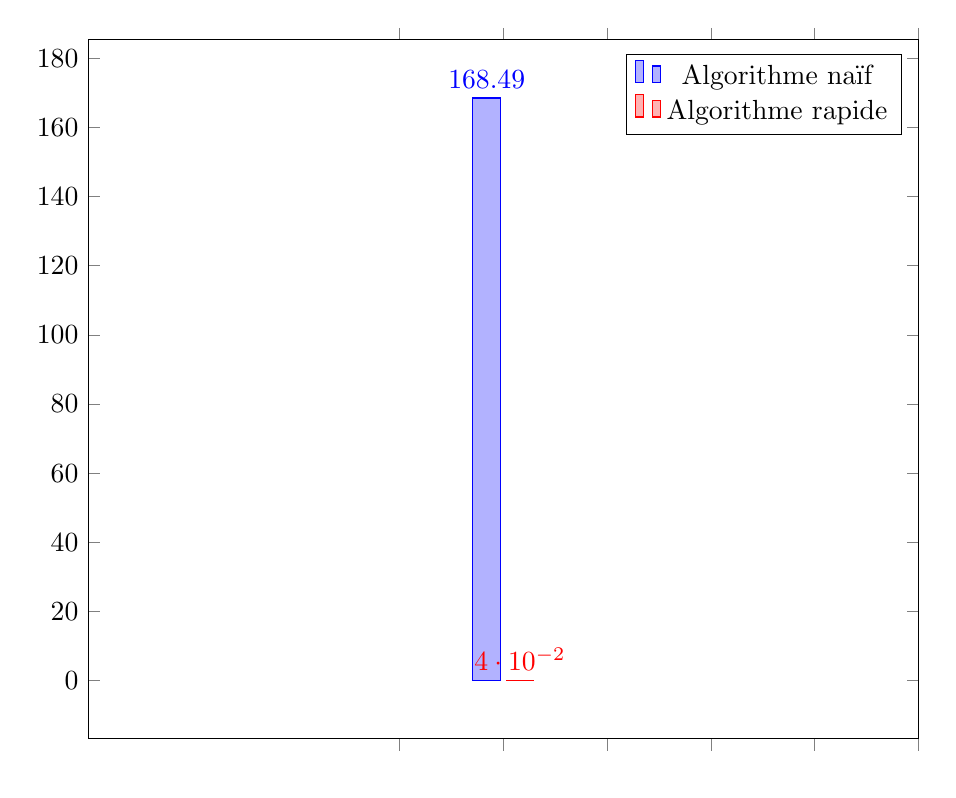
\begin{tikzpicture}
 
    \begin{axis} [
        ybar,
        nodes near coords,
        width=\textwidth,
        xticklabel=\empty
    ]
    \addplot coordinates {
        (1,168.49)
    };
    \addplot coordinates {
        (1,0.04)
    };
    \legend {Algorithme naïf, Algorithme rapide};
    \end{axis}

\end{tikzpicture}

\section{Écrire un programme de calcul des coefficients de Bézout}

\section{Écrire un programme de chiffrement RSA}